% Name: Area between two curves
% Description: The region between y = x and y = x²/3 from where they meet at x = 0 to where they meet at x = 3, with its area worked out.
% Tags: area between curves, definite integral, region, calculus

\usetikzlibrary{arrows.meta}

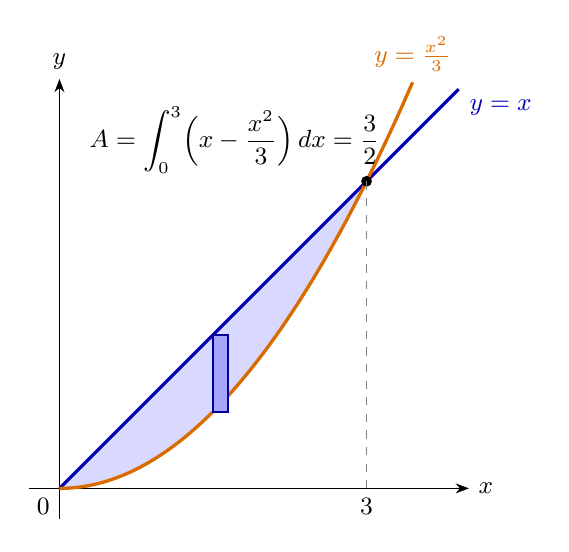
\begin{tikzpicture}[>={Stealth}, scale=1.3, every node/.style={font=\small}]
  \fill[blue!15] plot[domain=0:3, samples=40] (\x, \x) -- plot[domain=3:0, samples=40] (\x, {\x*\x/3}) -- cycle;
  \draw[->] (-0.3,0) -- (4,0) node[right] {$x$};
  \draw[->] (0,-0.3) -- (0,4) node[above] {$y$};
  \draw[very thick, blue!70!black, domain=0:3.9] plot (\x, \x) node[below right] {$y = x$};
  \draw[very thick, orange!85!black, domain=0:3.45, samples=40, smooth] plot (\x, {\x*\x/3}) node[above] {$y = \frac{x^2}{3}$};
  % A typical vertical strip, from the lower curve up to the upper one
  \draw[thick, blue!60!black, fill=blue!35] (1.5,0.75) rectangle (1.65,1.5);
  \fill (3,3) circle (1.5pt);
  \draw[dashed, gray] (3,3) -- (3,0) node[below, black] {$3$};
  \node[below left] at (0,0) {$0$};
  \node[anchor=west] at (0.2,3.4) {$\displaystyle A = \int_0^3 \Bigl(x - \frac{x^2}{3}\Bigr)\,dx = \frac{3}{2}$};
\end{tikzpicture}
